%!TeX program = xelatex
\documentclass[12pt,hyperref,a4paper,UTF8]{ctexart}
\usepackage{gzureport}

\usepackage{tabularx}
%%-------------------------------正文开始---------------------------%%
\begin{document}
%%-----------------------封面--------------------%%
\cover
%%------------------摘要-------------%%
%\begin{abstract}
%
%在此填写摘要内容
%
%\end{abstract}

\thispagestyle{empty} % 首页不显示页码

%%--------------------------目录页------------------------%%
\newpage
\tableofcontents

%%------------------------正文页从这里开始-------------------%
\newpage
\section{引言}

\subsection{图数据库技术的发展背景}

随着移动互联网时代发展, 数据量增长非常迅速, 并且数据类型也到得了进一步的扩展. 但是传统的关系型数据库在处理复杂关联关系时逐渐显现出其局限性: 关系型数据库通过表格化结构来进行数据建模, 然而在处理大量深度关联的数据时, 表格之间的多层外键连接操作使得查询变得非常复杂且耗时. 这对于实时、高效的应用场景而言是难以满足的, 特别是在社交网络、金融交易等需要处理大量关联数据的领域.

图数据库的出现则有效解决了这些问题. 图数据库以图论为理论基础, 将数据以节点和边的形式进行建模, 使得实体与实体之间的关系可以更加直观地进行表达. 这种建模方式不仅能够更高效地进行复杂关联关系的存储和查询, 还支持动态变化的数据结构. 在金融行业的反欺诈检测、社交网络中的关系分析等应用中, 图数据库凭借其优秀的性能逐渐成为一种重要的数据管理工具.

近年来, 随着对数据关联关系的深入挖掘, 图数据库得到了迅速的发展. 从最早的小规模原生图存储阶段 (Graph1.0) , 到当前支持大规模并行处理的图数据库 (Graph2.0和Graph3.0) , 图数据库的架构逐渐从单机部署演变为分布式架构, 查询效率和存储能力显著提升. 目前, 图数据库被广泛应用于知识图谱、社交网络、推荐系统、等多个领域, 成为了NoSQL数据库中重要的一个分支

\subsection{图数据库的提出与发展动因}

图数据库的提出与发展主要源于对复杂关联数据管理需求的不断增长. 传统的关系型数据库在处理多层次、多维度的数据关系时需要使用复杂的表连接操作, 这种操作随着数据量的增加会导致性能急剧下降. 例如, 当涉及多张表, 特别是复杂关联关系和大数据量时, 数据库需要对不同表之间的关系进行匹配和连接, 消耗大量的计算资源, 尤其是在深度连接时, 性能下降更为显著. 而在社交网络、电子商务、金融等领域, 数据的关联关系日益复杂, 传统数据库的建模方式和查询效率已经不能满足这些场景的需求.

与此同时, NoSQL数据库的兴起为解决结构化与非结构化数据存储问题提供了多样化的方案, 其中图数据库因其高效管理和存储关联关系数据的特性而受到关注. 与其他类型的NoSQL数据库 (如键值数据库、文档数据库) 相比, 图数据库的优势在于其在图结构上的高效性和灵活性, 能够处理关系紧密的数据集. 图数据库通过将实体 (节点) 和实体之间的关系 (边) 作为“一等公民”进行管理, 极大简化了复杂关联查询的实现.

此外, 社交网络、知识图谱、推荐系统等应用的普及也是图数据库迅速发展的重要驱动力, 因为这些领域的数据模型本质上是高度关联的网状结构, 图数据库在这些场景下具备显著的优势, 可以高效地表达、存储和查询数据中的复杂关系. 因此, 图数据库逐渐被应用于越来越多的场景, 并成为处理关联数据的核心工具.

图数据库的发展分为几个阶段, 最初的Graph1.0阶段是基于小规模原生图存储, 代表性产品是Neo4j的早期版本, 其主要存储规模限制在百万级节点和边. 随着大数据时代的到来, Graph2.0阶段的图数据库支持分布式存储和计算, 使得它们能够应对大规模的数据集, 例如JanusGraph和TigerGraph等, 实现了数十亿节点和边的存储与管理, 并显著提升了系统的扩展性和容错能力. 近年来, Graph3.0阶段的图数据库产品开始强调实时性和高并行计算能力, 进一步提升了查询性能, 使得实时复杂查询和分析成为可能, 同时支持更加复杂的计算任务的并行化处理, 例如内置的图算法库和支持多线程的并行计算.

\section{基本概念与核心特点}

\subsection{定义与数学基础}
图论是图数据库的理论基础, 如\autoref{fig:graph}所示. 图是由一组节点和连接这些节点的边组成的数学结构. 在图数据库中, 实体的每个特征可以作为节点的属性进行存储, 关系也可以具有属性. 这种方式使得图数据库能够直观地反映出实体之间的各种关系, 并通过图遍历等算法快速进行数据查询.

\begin{figure}[H]
	\centering
	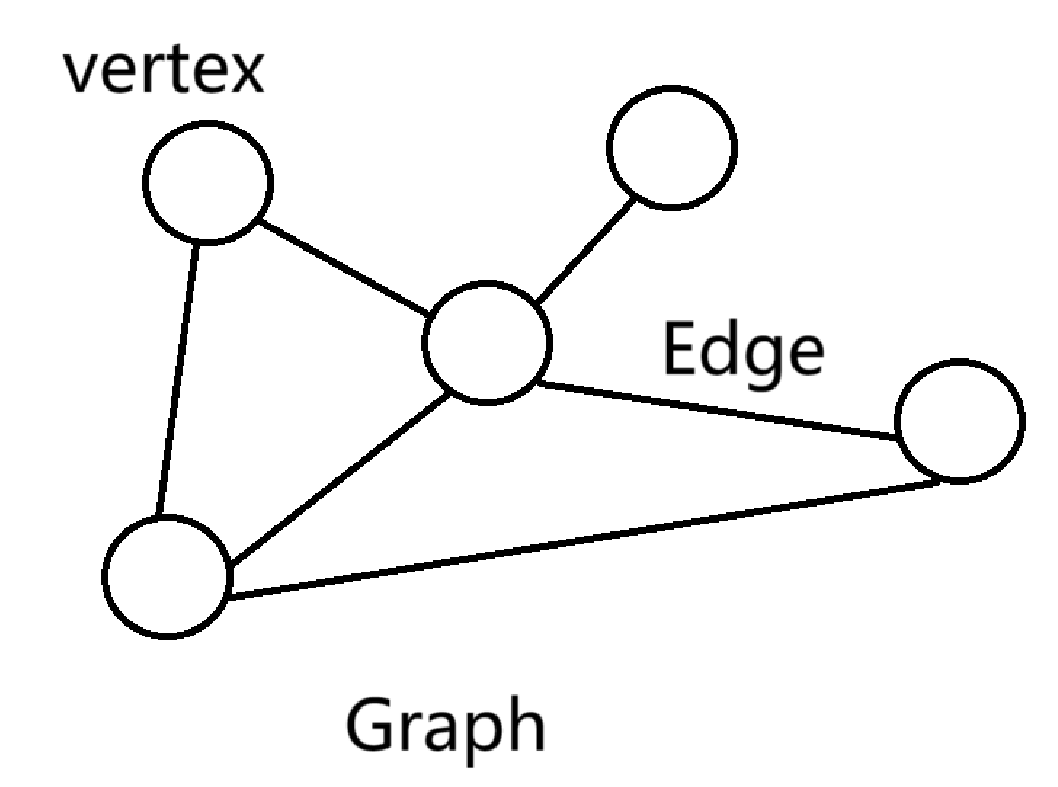
\includegraphics[width=0.8\textwidth]{images/7.png}
	\caption{Graph}
	\label{fig:graph}
\end{figure}
图数据库是一种用于管理和存储图结构数据的数据库管理系统, 以图论为理论基础进行数据建模. 图数据库中的基本单位是“节点 (Vertex) ”和“边 (Edge) ”, 其中节点用于表示实体, 边用于表示实体之间的关系. 与关系型数据库不同, 图数据库直接存储数据中的关系, 使得其能够更加自然和高效地表示复杂的数据结构. 例如, \autoref{fig:social-network}展示了一个简单的社交网络图, 其中节点代表用户, 边代表用户之间的好友关系. 图数据库能够直观地表示这种复杂的关系, 并通过图遍历等算法快速进行数据查询, 从而实现商品推荐,社区发现等上层应用.
\begin{figure}[H]
	\centering
	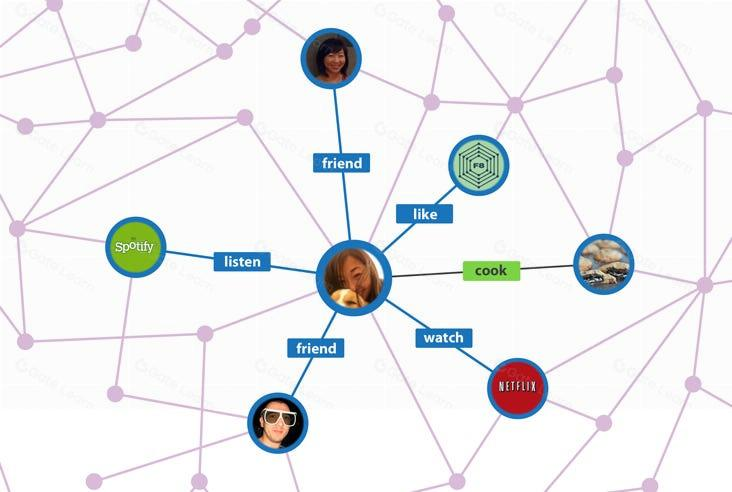
\includegraphics[width=0.8\textwidth]{images/8.png}
	\caption{社交网络}
	\label{fig:social-network}
\end{figure}


\subsection{主要模型}

图数据库主要有三种模型:

\textbf{属性图模型:} 属性图模型是图数据库中最常见的模型, 如\autoref{fig:property-graph}所示,其特点是节点和边都可以附带多个属性 (键值对) , 便于对复杂关系进行建模. 例如, 在社交网络中, 节点可以代表用户, 边可以代表好友关系, 而属性则可以存储用户的年龄或好友关系的建立时间. 属性图模型的优点是灵活且直观, 适合表示复杂的实体和关系, 查询效率高. 但其对于高度结构化的数据, 可能没有关系型数据库的存储和处理效率高.
\begin{figure}
	\centering
	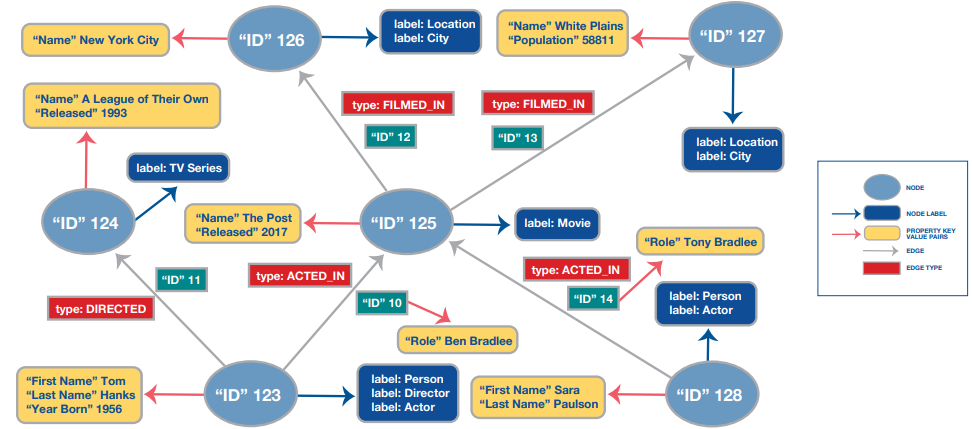
\includegraphics[width=\textwidth]{images/9.png}
	\caption{属性图模型}
	\label{fig:property-graph}
\end{figure}

\textbf{资源描述框架模型:} 资源描述框架(Resource Description Framework, RDF) 模型基于W3C提出的标准, 适用于语义网络应用. 如图\autoref{fig:rdf}, 它使用三元组 (主语-谓语-宾语) 来表示数据. 例如, “Alice 是 Bob 的好友”可以表示为一个三元组. 这种模型广泛应用于语义网和知识图谱中. RDF模型的优点在于标准化程度高, 特别适合构建可扩展的语义网络, 数据互操作性好;但是其存储结构较为冗长, 对于复杂关系的查询性能可能不如属性图模型高.
\begin{figure}[H]
	\centering
	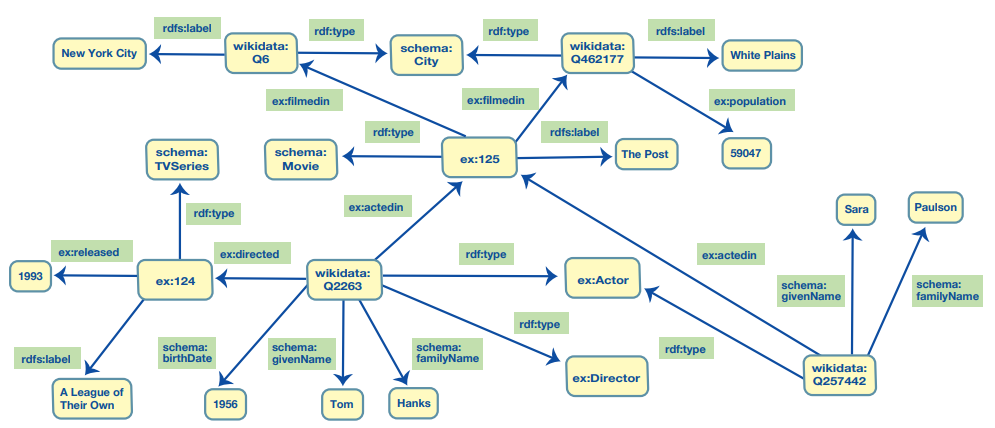
\includegraphics[width=\textwidth]{images/10.png}
	\caption{资源描述框架模型}
	\label{fig:rdf}
\end{figure}

\textbf{超图模型:} 超图是节点与一组节点之间关系的扩展, 适用于表示复杂多方关系的场景. 例如, 一个项目小组可以表示为一个超边, 连接多个节点 (即组内成员) . 超图模型的优点是能够更加方便地表示多对多的关系, 适合描述复杂的群体交互场景;但其实现复杂度较高, 查询操作也可能比其他图模型更加复杂, 导致查询效率受到影响.



\subsection{与关系型数据库的比较}

图数据库与传统关系型数据库相比, 具有显著的特点和优势.

\textbf{建模方式:} 关系型数据库使用“表格化结构”来表示数据, 适合处理结构化数据. 但当数据之间存在复杂的多层次关联关系时, 需要使用外键进行多次表连接, 导致查询效率下降. 而图数据库通过“节点-边”的建模方式, 可以更自然地表达复杂的关联关系.
\begin{figure}[H]
	\centering
	\begin{subfigure}[b]{0.45\textwidth}
		\centering
		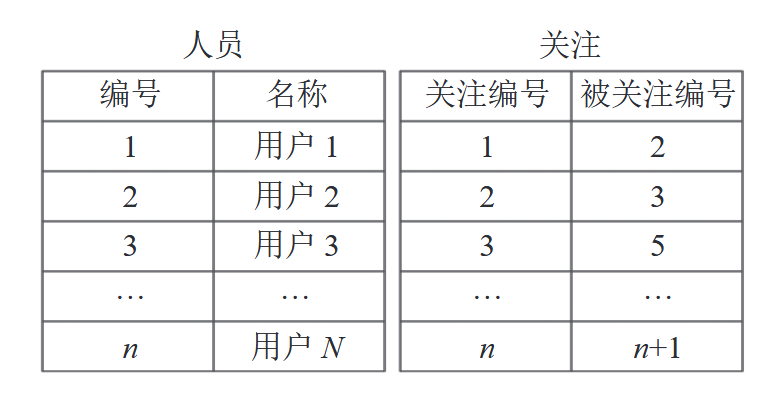
\includegraphics[width=\textwidth]{images/1.png}
		\caption{关系型数据库}
	\end{subfigure}
	\hfill
	\begin{subfigure}[b]{0.45\textwidth}
		\centering
		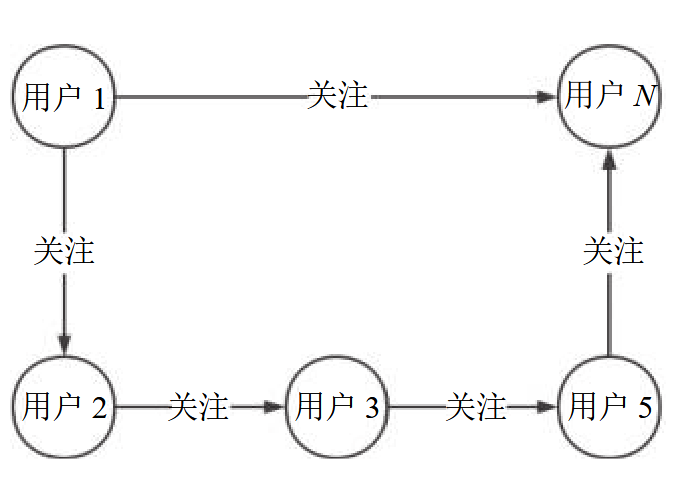
\includegraphics[width=\textwidth]{images/2.png}
		\caption{图数据库}
	\end{subfigure}
\end{figure}


\textbf{查询效率:} 在涉及深度关联的查询中, 关系型数据库需要通过多次JOIN操作进行表的关联, 查询的复杂度和时间消耗迅速增加. 而图数据库则可以通过图遍历的方式, 直接在节点和边之间进行跳转, 大幅提高查询效率.

\textbf{灵活性:} 图数据库具有灵活的数据模式, 支持在不影响现有数据的情况下对数据模型进行扩展. 这种灵活性使得图数据库在面对动态变化的数据结构时, 能够更轻松地进行更新和维护.

\section{组成架构}

\subsection{接口层: API与查询语言}

接口层是用户与图数据库系统之间的交互接口, 主要包括API和查询语言. API (应用程序接口) 使得开发者可以通过编程语言与数据库进行交互, 执行各种操作, 如增、删、改、查等. 图数据库通常支持多种查询语言, 如Neo4j的Cypher语言、Apache TinkerPop的Gremlin等. 这些查询语言使得用户能够方便地对图数据进行复杂的查询和分析. 接口层的设计直接关系到系统的易用性和灵活性.

\subsection{计算层: 查询引擎与优化器}

计算层负责处理用户的查询请求, 包括查询的解析、优化和执行. 查询引擎接收用户通过接口层提交的查询请求, 并将其转化为可以执行的查询计划. 优化器则对查询计划进行优化, 以提高查询的执行效率. 图数据库的查询引擎需要处理大量节点和边的遍历, 因此其性能在很大程度上决定了数据库的整体表现. 高效的查询引擎和优化器是保证复杂图查询能够在合理时间内完成的关键.

\begin{figure}[H]
	\centering
	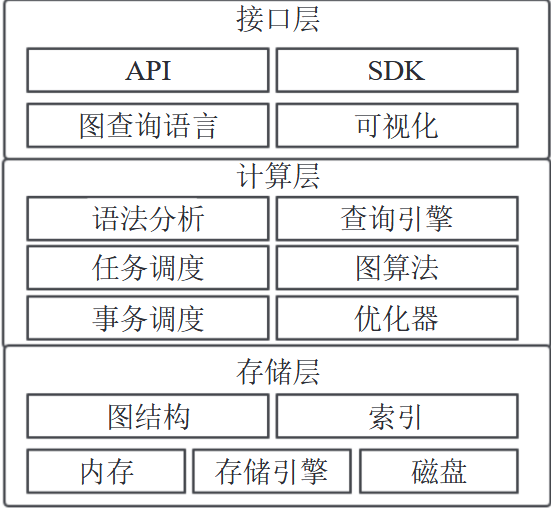
\includegraphics[width=0.6\textwidth]{images/3.png}
	\caption{图数据库的组成架构}
\end{figure}

\subsection{存储层: 原生图存储与非原生图存储}

存储层是图数据库的基础, 负责存储节点、边及其属性. 根据实现方式的不同, 图数据库的存储层可以分为原生图存储和非原生图存储.
原生图存储是专门为图数据设计的存储结构, 能够直接以图的形式存储数据, 查询时可以高效地进行节点和边的遍历操作, 代表性的产品有Neo4j. 这种存储方式能够充分利用图数据的特性, 提供高效的存储和查询性能.
非原生图存储则是基于已有的通用数据库系统 (如关系型数据库或键值存储) 实现的图存储. 这种方式通过将图数据映射到关系型表格或键值对中来进行存储, 虽然实现成本较低, 但在查询图结构数据时效率较低, 典型的产品有JanusGraph. 这种存储方式适合一些对查询效率要求不高, 或已有存储系统需要扩展支持图数据的场景.

\section{关键技术详解}

\subsection{存储}

图数据库的存储技术是其核心组成之一, 直接影响到数据库的性能和扩展性. 图数据库存储方式包括原生图存储和非原生图存储.

\subsubsection*{原生图存储}

原生图存储是专门为图数据而设计的存储方式, 能够自然地存储节点、边及其属性. 由于原生图存储以图为基本单元, 存储结构和图的物理结构保持一致, 因此可以直接、高效地进行节点间的遍历操作. 原生图存储通常采用\textbf{邻接列表或邻接矩阵}作为其底层数据结构.

邻接列表是一种常见的图数据存储方式,如\autoref{fig:adjacency-list}所示, 对于每个节点, 存储一个列表以记录其相邻节点. 邻接列表的优势在于存储空间效率高, 特别适用于稀疏图, 因为只需存储存在的边. 其劣势在于, 当需要快速查找两个节点之间的关系时, 可能需要遍历整个邻接列表.
\begin{figure}[H]
	\centering
	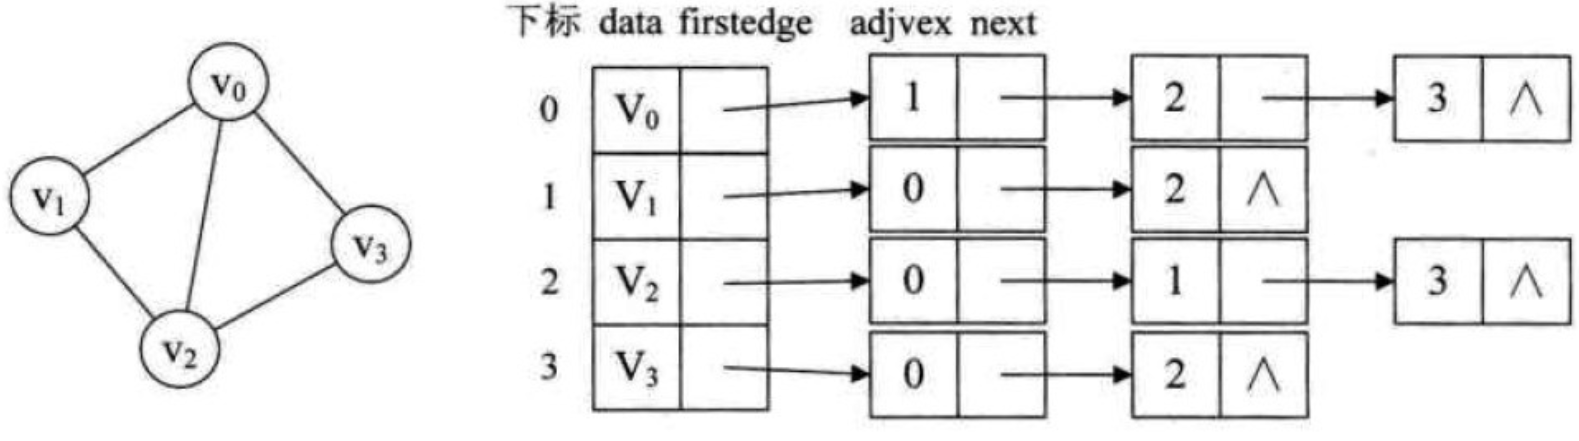
\includegraphics[width=1\textwidth]{images/11.png}
	\caption{邻接列表}
	\label{fig:adjacency-list}
\end{figure}

Neo4j是最具代表性的原生图数据库, 其存储引擎专门针对图遍历进行了优化, 使得复杂关系查询的性能得以保障.如\autoref{fig:neo4j}所示, Neo4j的存储方式结合了指针和嵌入式存储, 使得在遍历节点和边时可以实现低延迟的高效访问.
\begin{figure}[H]
	\centering
	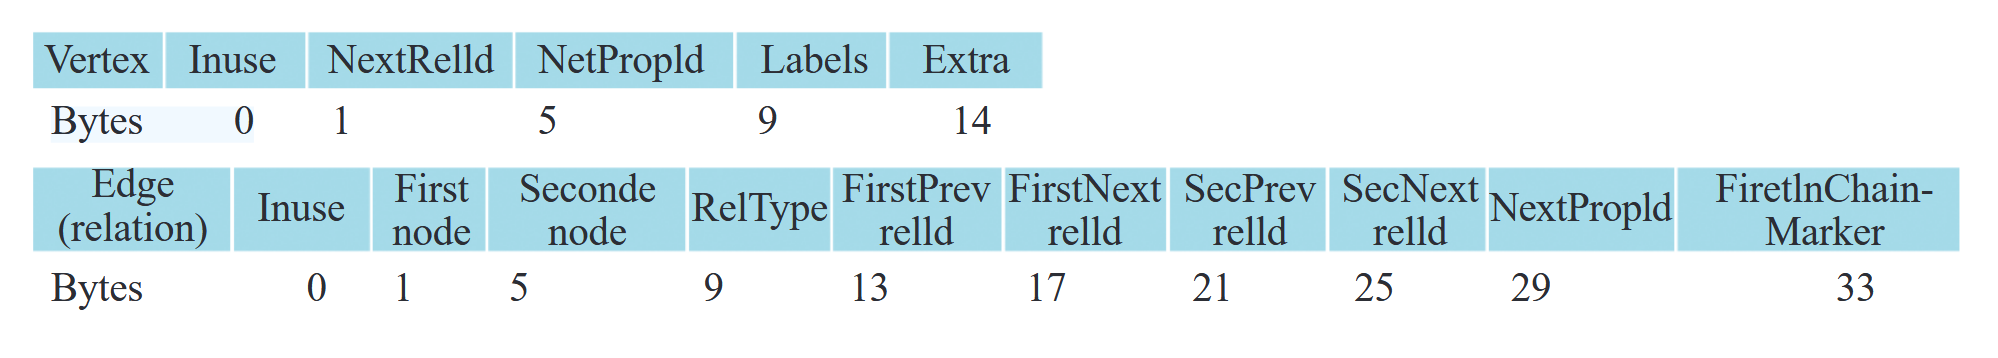
\includegraphics[width=1\textwidth]{images/4.png}
	\caption{Neo4j的存储结构}
	\label{fig:neo4j}
\end{figure}

\autoref{tab:neo4j-vertex}展示了Neo4j中节点的存储结构, 其中包括节点的有效性、关联关系的指针、标签等信息.
\begin{table}[H]
	\centering
	\caption{Neo4j的vertex存储结构}
	\begin{tabular}{|c|c|c|}
		\hline
		顶点字段       & 字节位置 & 说明              \\
		\hline
		iussu      & 0    & 是否有效            \\
		NextRelI   & 1-4  & 关联到该节点的第一个关系的id \\
		NextPropId & 5-8  & 关联到该节点的第一个属性的id \\
		labels     & 9-12 & 指向标签的指针         \\
		Extra      & 13   & 存储内部标志信息        \\
		\hline
	\end{tabular}
	\label{tab:neo4j-vertex}
\end{table}
Neo4j通过其独特的存储结构实现了高效的图数据处理能力。在节点存储方面,Neo4j采用了紧凑的13字节结构,其中包含了关键的NextRelI字段用于存储第一个关联关系的ID,为快速图遍历提供了入口点。同时,NextPropId字段直接链接到节点的属性存储,实现了属性的快速访问,而labels字段则通过直接指针定位标签信息,避免了额外的查找开销。这种紧凑的存储结构不仅节省了存储空间,更重要的是提高了缓存效率。


\autoref{tab:neo4j-edge}展示了Neo4j中边的存储结构, 包括边的有效性、起始节点和终止节点的id、边的类型等信息. 通过这种存储方式, Neo4j能够高效地存储和查询图数据, 并支持复杂的图遍历操作.
\begin{table}[H]
	\centering
	\caption{Neo4j的Edge存储结构}
	\begin{tabular}{|c|c|c|}
		\hline
		顶点字段              & 字节位置  & 说明             \\
		\hline
		iussu             & 0     & 是否有效           \\
		firstNode         & 1-4   & 关系的起始节点id      \\
		secondNode        & 5-8   & 关系的终止节点id      \\
		relType           & 9-12  & 关系的类型          \\
		firtPrevRelId     & 13-16 & 指向起始顶点上前一个边的指针 \\
		firtNextRelId     & 17-20 & 指向起始顶点上后一个边的指针 \\
		secPrevRelId      & 21-24 & 指向终止顶点上前一个边的指针 \\
		secNextRelId      & 25-28 & 指向终止顶点上后一个边的指针 \\
		nextProId         & 29-32 & 边记录第一个属性的id    \\
		fristinChainMaker & 33-36 & 是否为关系链的第一条边    \\
		\hline
	\end{tabular}
	\label{tab:neo4j-edge}
\end{table}
在边的存储结构设计上,Neo4j采用了更为复杂的机制。通过firstPrevRelId、firstNextRelId等字段构建的双向链表结构,使得系统能够高效地在相关节点间进行双向遍历。边存储直接包含了起始和终止节点的ID,避免了间接寻址带来的性能损耗。同时,relType字段的设计支持关系类型的快速过滤,而firstinChainMaker的标记则有助于关系链的快速识别和处理。这种存储结构使得图的遍历操作能够保持较低的延迟。

原生图存储的优势在于针对性强, 能够充分利用图结构的特性来提供高效的存储和检索能力, 尤其在复杂关系密集的场景中表现优异. 然而, 其缺点是对分布式扩展支持有限, 难以适应超大规模数据场景下的高效水平扩展.



\subsubsection*{非原生图存储}

非原生图存储是基于已有的通用数据库 (如键值存储) 来支持图数据存储的方案. 如\autoref{fig:janusgraph-vertex}所示,这种存储方式通过将节点和边映射到表或键值对中进行存储, 常用的数据结构包括关系表和键值对映射.
\begin{figure}[H]
	\centering
	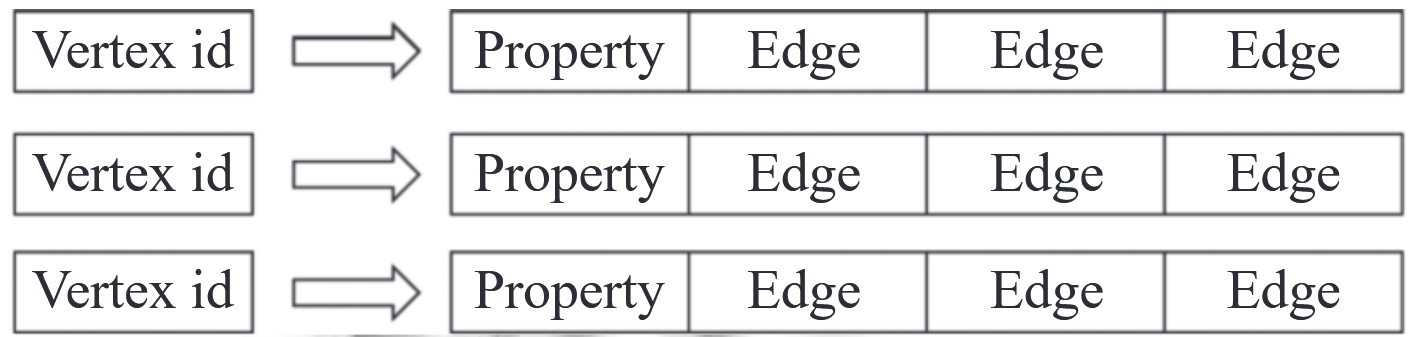
\includegraphics[width=\textwidth]{images/6.png}
	\caption{非原生图存储}
	\label{fig:non-native}
\end{figure}
\autoref{fig:janusgraph-vertex}展示了JanusGraph的Vertex存储结构,其中vertex id 共包含一个字节, 8 位, 64 bit, 分为  3 个部分: partition id、count、ID padding. 前 5 位为partition id, partition 是 JanusGraph 抽象出的概念, 通过  其数量计算可以最终使数据均匀分配到多台机器中.  中间的 count 是流水号, 最高位固定为 0, 其剩余位数  足以生成 2 的 55 次幂个 id, 满足节点数量生成. 最后几位 bit 是 ID padding, 表示 Vertex 的类型, 具体位数长度会随不同类型有所修改, 常用情况值为“000”.
\begin{figure}[H]
	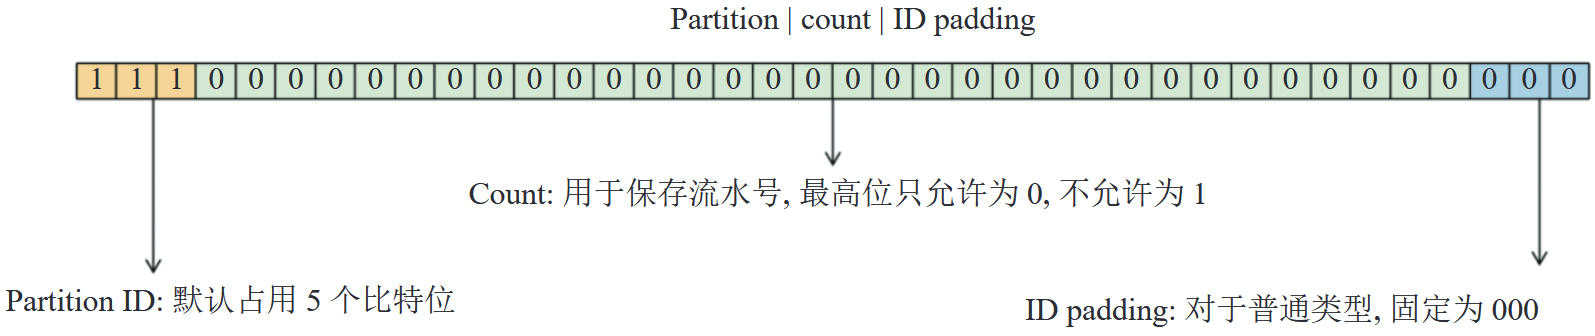
\includegraphics[width=1\textwidth]{images/12.png}
	\caption{JanusGraph的Vertex存储结构}
	\label{fig:janusgraph-vertex}
\end{figure}
\autoref{fig:janusgraph-edge}给出了 Edge 和 Property 的逻辑结构, 均分别由 column 和 value 两部分组成. 在 Edge 的 column 中, 包含了 label id、direction, sort key、adjacent vertex id 和 edge id. 其中, label id 是边类型代表的 id. Direction 是图的方向, 用0和1来分别代表出和入. Sort key可以指定多个边的属性. Adjacent vertex id 是目标节点 id, 实际存储的是目标节点id和源节点 id 的差值. Edge id 则是边的全局唯一 id. Edge的 value由 signature key 和 other property 组成, 前者用于提升 edge 的属性的检索速度, 后者则是存储边的其他属性.  Property 的 column 包含 key id 和 property id, 前者用于存储属性 label 对应的 id 值, 后者则是指定属性的唯一 id. Value 中只有 property value用于保存属性值
\begin{figure}[H]
	\centering
	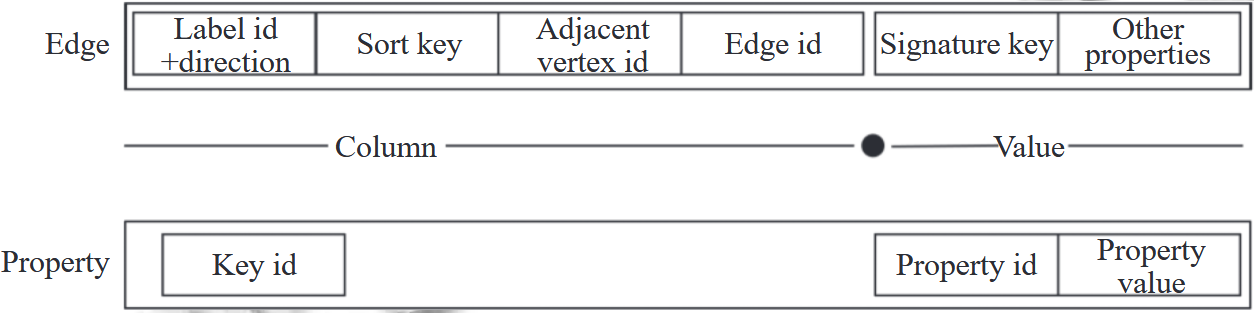
\includegraphics[width=0.8\textwidth]{images/13.png}
	\caption{JanusGraph的Edge存储结构}
	\label{fig:janusgraph-edge}
\end{figure}

非原生图存储的优点在于扩展性强, 可以利用已有数据库系统的可靠性和分布式能力, 适合超大规模数据存储的需求;但由于其底层并非针对图结构优化, 因此在图遍历和复杂查询方面性能有限, 尤其在深度查询和多跳查询的情况下表现不如原生存储高效.

\subsection{查询}

图数据库的查询功能是其核心优势之一, 通过查询语言和算法的结合, 使得用户能够高效地从图中获取信息. 图数据库的查询主要包括命令式查询语言、声明式查询语言以及支持的图遍历和分析算法.

\subsubsection*{命令式查询语言}

命令式查询语言要求用户明确指定如何执行查询操作, 包括每一步遍历和过滤的详细指令. Apache TinkerPop的Gremlin是一个典型的命令式查询语言, 其查询风格类似于编程, 用户需要指定每一步的节点或边的操作. Gremlin适合灵活、复杂的查询需求, 但对用户的编程能力要求较高. 通过命令式查询, 用户可以对图数据进行逐步遍历, 从而实现复杂的多跳查询和条件筛选.

例如, 假设我们有一个社交网络图数据库, 其中节点代表用户, 边代表好友关系. 要查找某个用户的好友的好友, 可以使用以下Gremlin查询:

\tbox{g.V().has('name', 'Alice').out('knows').out('knows').values('name')}

这段代码的含义是: 找到名称为“Alice”的节点, 然后遍历其所有的“knows”关系, 接着再遍历这些好友节点的“knows”关系, 最后返回这些好友的好友的名称.

\subsubsection*{声明式查询语言}

声明式查询语言则让用户关注“要查询什么”而不是“如何查询”. Neo4j的Cypher语言就是一种典型的声明式查询语言. Cypher通过类似SQL的语法, 用户可以方便地描述想要查询的图结构和条件, 而无需指定遍历的细节. Cypher语法简洁, 易于学习, 对于常见的查询需求如模式匹配和路径查找非常高效. 例如, 在社交网络图数据库中, 假设我们要查找名称为“Alice”的用户的好友, 可以使用以下简单的一行Cypher查询语句:

\tbox{MATCH (a:Person {name: 'Alice'})-[]->(friend) RETURN friend.name}

声明式查询语言的优势在于易用性强, 用户可以快速上手并实现复杂的查询, 而无需了解底层遍历细节. 这对于大多数应用场景是非常友好的, 尤其在社交网络和推荐系统中, Cypher被广泛应用.

\subsubsection*{Cypher、Gremlin、GSQL介绍与对比}
Cypher、Gremlin和GSQL是图数据库领域最常见的三种查询语言, 各有优缺点.
% Table generated by Excel2LaTeX from sheet 'Sheet1'
\begin{table}[htbp]
	\centering
	\caption{三种图查询语言对比}
	\begin{tabularx}{\textwidth}{|X|X|X|X| }
		\hline
		查询语言  & Cypher                       & Gremlin              & GSQL                \\
		\hline
		提出者   & Neo4j                        & Apache TinkerPop     & TigerGraph          \\
		\hline
		介绍    & 类SQL,开源版本为OpenCypher         & 类Scala               & 类SQL,支持Map-Ruduce模型 \\
		\hline
		图灵完备性 & SQL完备(结合SDK可以图灵完备)           & 图灵完备                 & 图灵完备                \\
		\hline
		使用的产品 & Neo4j-AgensGraph、RedisGraph等 & OrientDB、JanusGraph等 & TigerGraph          \\
		\hline
	\end{tabularx}%
	\label{tab:addlabel}%
\end{table}%

Cypher: 是一种声明式语言, 强调简洁和可读性, 适合新手和非技术人员. Cypher非常适合对图进行模式匹配和简单查询, 易用性是其主要优势.

Gremlin: 是一种命令式语言, 具有高度的灵活性, 适合对图数据进行复杂的逐步遍历. Gremlin的优势在于灵活性高, 但学习曲线较陡, 适合需要复杂自定义查询的场景.

GSQL: 是TigerGraph开发的一种图查询语言, 结合了声明式和命令式的优点, 支持复杂的图分析和并行计算, 尤其适用于大规模数据和复杂分析场景. GSQL能够以类似编程语言的方式进行复杂逻辑的编写, 并且在分布式图计算中表现优秀.

三者在实际使用中的选择取决于应用场景和用户需求: 对于快速实现常见查询, Cypher是最佳选择;对于需要更高灵活性的逐步遍历, Gremlin较为合适;而在需要大规模并行处理和复杂分析的情况下, GSQL则表现出色.

\subsection{图算法}

图算法是图数据库的核心工具之一, 用于分析和提取图中的有用信息. 图数据库通常内置了多种图算法, 这些算法可以分为实时查询和离线分析两大类, 分别用于解决不同场景下的图数据问题.

\textbf{图遍历}: 图遍历是一种基础的图操作, 用于访问图中的所有节点和边. 常见的图遍历方法有深度优先遍历 (DFS) 和广度优先遍历 (BFS) . 这些遍历方法被广泛应用于图的搜索、路径查找等任务. 在图数据库中, 遍历操作是执行复杂查询的基础, 例如查找特定条件下的路径或识别满足特定关系链的节点.

\textbf{最短路径算法}: 最短路径算法用于查找图中两个节点之间的最短路径, 通常应用于寻找最优路线或最小成本路径的场景. 例如, Dijkstra算法是一种经典的最短路径算法, 适用于图中的加权边, 用于查找从一个起始节点到其他节点的最短路径. 在图数据库中, 最短路径算法常用于社交网络中查找两个人之间的最短关系链, 或在物流系统中查找最优运输路线.

\textbf{PageRank算法}: PageRank算法最初是为搜索引擎排名设计的, 主要用于衡量节点在图中的重要性. 该算法通过计算节点间相互链接的数量和质量, 来确定每个节点的重要程度. 在图数据库中, PageRank算法常被用于社交网络中确定用户的影响力、在引用网络中衡量学术文章的影响力, 或者在推荐系统中识别重要的产品或用户.

\textbf{社区发现算法}:社区发现算法用于识别图中密切关联的节点集合, 即“社区”. 这些算法能够有效地找出具有强连接特征的子图, 例如社交网络中的兴趣小组, 或生物网络中具有相似功能的基因群. 常见的社区发现算法包括Girvan-Newman算法和Louvain算法. 社区发现有助于了解图中节点的聚类特性, 从而用于推荐、群体分析等应用.

\textbf{连通组件算法}: 连通组件算法用于查找图中相互连通的所有节点集合. 对于无向图, 连通组件是图中所有节点之间直接或间接连接的最大集合. 连通组件算法在社交网络分析中应用广泛, 用于检测用户群体, 或者在网络安全中用于检测恶意节点群体.



\subsection{实时查询}

图数据库中的实时查询依赖于高效的图遍历和路径计算, 例如实时路径查找、推荐好友或发现潜在的关系. 实时查询通常需要在短时间内返回结果, 因此对查询的性能要求较高. 为了实现毫秒级的查询响应,图数据库系统采用了多种优化技术来提升查询性能

\textbf{索引机制}: 为了加速节点和边的查找过程, 图数据库通常为节点属性和关系创建索引. 通过使用索引, 查询可以在大量节点中快速定位到目标节点, 而无需遍历所有节点. 这显著减少了查找时间. 例如,在社交网络中查找特定年龄段的用户时,通过年龄属性索引可以直接定位目标用户群体,而无需遍历整个用户图。索引的选择和维护需要在存储开销和查询性能之间取得平衡,因此图数据库通常提供自适应索引机制,能够根据查询模式动态调整索引策略

\textbf{缓存技术}: 图数据库通常会利用缓存技术存储常用的查询结果和中间计算结果, 从而避免重复计算. 这意味着, 对于常见的查询可以直接从缓存中读取结果, 从而减少了查询的响应时间. 例如,热点节点缓存,将热点节点及其邻居信息维护在内存中,提供快速访问,或者是使用路径缓存,保存常用的路径计算结果,特别适用于社交网络中的"共同好友"等查询


\textbf{并行化处理}: 在处理复杂图查询时, 图数据库会将任务拆分为多个子任务并行执行. 例如, 当需要查找多条路径或执行复杂的模式匹配时, 这些任务可以分配到不同的计算单元来同时处理. 并行化处理能够显著提高查询的效率, 缩短返回结果的时间.

\textbf{最短路径索引}: 对于经常查询最短路径的应用场景, 图数据库可以提前构建最短路径索引, 这样在执行最短路径查询时可以直接使用预计算的数据, 从而加速查询的返回时间.

以上技术虽然需要额外的存储空间,计算和维护开销,但能显著提升路径查询的性能。通过这些优化技术的组合应用,现代图数据库能够在保证数据一致性的同时,提供高效的实时查询服务。这些技术相互配合、互为补充,形成了一个完整的性能优化体系。

\subsection{离线分析}

离线分析则主要应用于大规模的图数据分析任务, 例如社交网络中的社区检测、大规模的节点排序等. 这些分析任务通常是批处理的, 时间要求相对宽松, 但计算量较大, 需要充分利用分布式计算资源. 为了有效处理这些复杂的分析任务,图数据库系统采用了一系列专门的技术和框架。这些技术主要从数据存储、计算框架和并行处理等方面入手,构建起完整的离线分析体系。

\textbf{分布式存储}: 分布式存储是大规模图数据处理的基础设施。在实际应用中,图数据通常会按照特定的策略进行分区,如边切分或顶点切分,每个分区被分配到不同的存储节点上。为了提高数据访问效率,系统会考虑图的拓扑结构进行数据放置,尽量将紧密关联的节点和边存储在同一个分区内。例如,在社交网络分析中,同一个社交圈子的用户数据会倾向于存储在相同或邻近的存储节点上。此外,分布式存储系统通常会实现数据复制机制,在多个节点上保留数据副本,这不仅提高了数据的可用性,也为并行数据访问提供了可能。存储系统还会维护分布式索引,帮助快速定位数据所在的物理位置,减少跨节点数据访问的开销。例如,当需要分析用户群体的兴趣特征时,系统可以并行地从不同存储节点读取用户数据,大大提高数据加载的效率。

\textbf{分布式计算框架}: 图数据的分布式计算框架通常采用迭代计算模型,将复杂的图分析任务分解为多轮迭代执行的简单操作。在每轮迭代中,计算任务被划分为映射(Map)和归约(Reduce)两个阶段。在映射阶段,每个计算节点独立处理分配给它的图数据子集,执行诸如节点值更新、边权重计算等局部操作。在归约阶段,系统将各个节点的中间结果进行合并,完成全局计算。例如,在计算社交网络的影响力分数时,每个计算节点首先处理其负责的用户子集的直接关系网络,然后通过多轮迭代逐步扩展影响范围,最终汇总得到全局的影响力评分。为了提高计算效率,框架会实现智能的任务调度策略,根据数据分布和节点负载动态调整计算任务的分配。同时,框架还提供容错机制,能够处理节点故障等异常情况,确保大规模计算任务的可靠完成。

\textbf{并行图计算框架}: 专门的并行图计算框架采用"以顶点为中心"或"以边为中心"的计算模型,针对图数据的特殊结构提供了更高效的并行处理机制。这类框架通常维护一个全局的同步点,确保所有计算节点在每轮迭代中保持同步,从而保证计算结果的正确性。在实际应用中,框架会根据具体算法的特点选择适当的并行策略。例如,在进行社区检测时,可能采用异步的消息传递机制,允许不同社区的检测过程以不同的速度推进,从而提高整体的计算效率。框架还实现了高效的数据分区和通信机制,通过最小化节点间的数据交换来提升性能。例如,在计算最短路径时,框架会优先处理本地数据,只在必要时才进行跨节点的路径信息交换。为了处理超大规模图数据,一些框架还支持外存计算,能够有效管理无法完全装入内存的图数据,通过优化的磁盘访问策略来维持较好的计算性能。

通过以上技术和框架的配合,共同提升图数据库在离线分析计算上的性能
\section{主流产品}

\subsection{Neo4j}

Neo4j 是当前最流行的图数据库之一, 最早在 2007 年推出, 其设计之初即为原生图数据库. Neo4j 采用属性图模型, 以节点 (Node) 、边 (Relationship) 和属性 (Property) 的形式来存储和表示数据. 它使用 Cypher 作为主要的查询语言, 这种声明式查询语言使得复杂关系的查询非常简洁和直观.

Neo4j 的主要特点包括:

\textbf{原生图存储}: Neo4j 采用原生图存储技术, 能够高效地存储和遍历节点与边, 这使得其在复杂关联关系的查询中表现出色.

\textbf{高效的查询引擎}: 通过 Cypher 查询语言, Neo4j 可以实现复杂图形数据的模式匹配, 适合社交网络分析、知识图谱等领域.

\textbf{应用场景}: Neo4j 被广泛用于社交关系分析、推荐系统、欺诈检测等场景, 尤其在需要快速返回结果的实时查询任务中表现出色.

Neo4j 在复杂数据建模和实时查询上具有显著优势, 但由于其单节点架构, 其在分布式和水平扩展方面存在一定的局限性.

\subsection{TigerGraph}

TigerGraph 是一款专为大规模图计算设计的分布式图数据库, 特别擅长处理大规模数据集和复杂图分析. TigerGraph 支持原生的分布式图存储架构, 并采用 GSQL 作为主要的查询语言. GSQL 结合了声明式和命令式的特性, 具有较高的灵活性和可扩展性.

TigerGraph 的主要特点包括:

\textbf{分布式存储与计算}: TigerGraph 采用分布式存储架构, 能够处理数十亿节点和边的数据, 支持大规模并行计算.

\textbf{高效的图分析能力}: TigerGraph 内置了多种图算法 (如 PageRank、最短路径等) , 并通过并行化处理显著提高了分析效率, 适合离线大规模图分析任务.

\textbf{应用场景:} TigerGraph 在金融欺诈检测、物联网、企业知识图谱和供应链管理等领域应用广泛, 特别是在需要对大规模数据进行复杂分析的情况下表现优异.

TigerGraph 的优势在于其出色的扩展能力和并行计算性能, 但 GSQL 的学习曲线相对较陡, 对用户的技术要求较高.

\subsection{JanusGraph}

JanusGraph 是基于 Apache TinkerPop 框架的一个开源分布式图数据库, 专门设计用于大规模图数据的存储和管理. JanusGraph 支持多种后端存储 (如 HBase、Cassandra 等) , 并通过整合现有的 NoSQL 数据库来管理图数据.

JanusGraph 的主要特点包括:

\textbf{可扩展的分布式架构}: 通过集成多种后端存储, JanusGraph 能够处理大规模的图数据, 具有较强的扩展性和分布式处理能力.

\textbf{灵活的后端支持}: 用户可以根据需求选择不同的后端存储, 如键值数据库或列族数据库, 这为系统的灵活部署提供了更多选择.

\textbf{查询语言与图遍历}: JanusGraph 使用 Gremlin 作为主要查询语言, Gremlin 的命令式风格使得其在需要灵活控制查询步骤的场景中表现良好.

JanusGraph 的优点在于其良好的分布式支持和灵活性, 适合部署在已有的分布式数据库基础设施上, 但由于其非原生的图存储架构, 在查询性能上不如 Neo4j

\subsection{对比}



\begin{table}[htbp]
	\centering
	\caption{图数据库比较}
	\begin{tabularx}{\textwidth}{|X|X|X|X|}
		\hline
		\textbf{特性} & \textbf{Neo4j} & \textbf{TigerGraph} & \textbf{JanusGraph} \\
		\hline
		存储架构        & 原生图存储          & 原生分布式图存储            & 基于后端的非原生图存储         \\
		\hline
		查询语言        & Cypher (声明式)   & GSQL (结合声明式与命令式)    & Gremlin (命令式)       \\
		\hline
		扩展性         & 单节点为主, 扩展性有限   & 高度可扩展, 支持大规模数据      & 通过后端支持, 具备分布式能力     \\
		\hline
		查询性能        & 对于复杂关系查询性能优秀   & 高效并行计算, 适合大规模分析     & 依赖后端存储, 查询性能受限      \\
		\hline
		典型应用场景      & 社交网络、推荐系统      & 金融欺诈检测、供应链管理        & 大规模知识图谱、灵活部署场景      \\
		\hline
		复杂分析能力      & 支持多种图算法, 但非并行化 & 内置并行图算法, 适合离线分析     & 通过 Gremlin 进行复杂图计算  \\
		\hline
	\end{tabularx}
	\label{tab:graph_comparison}
\end{table}

Neo4j 适用于实时查询和快速开发需求, 尤其是在单机部署和需要直观声明式查询的场景中.
TigerGraph 在大规模并行计算和复杂图分析方面表现出色, 适合对海量数据进行深入分析的场景.
JanusGraph 则更加灵活, 适合整合已有的分布式存储系统, 尽管在查询性能上可能不如其他原生图数据库.
对于需要大规模并行处理的企业知识图谱, TigerGraph 是最佳选择. 而对于快速开发和灵活查询需求, Neo4j 更为合适. JanusGraph 则适合那些已有分布式存储系统并希望扩展为图数据存储的用户

\section{实际应用案例}

\subsection{社交网络分析}
图数据库在社交网络分析中被广泛应用,其核心特性是能够直观地存储和高效地查询节点之间的复杂关系。在社交网络中,用户被表示为节点,用户之间的社交关系(如好友关系、关注关系)被表示为边,这使得图数据库能够自然地建模并高效管理这些数据。

\textbf{好友推荐}:图数据库如 Neo4j 能够通过遍历社交图,实时地向用户推荐新的朋友。利用 Cypher 查询语言,Neo4j 可以在极短的时间内找到用户的好友的好友,计算可能认识的人,从而实现好友推荐功能。例如,在 Facebook 的社交网络中,实时推荐基于节点之间的距离和共同好友数\cite{ahmad2020missing,wang2022common}。

\textbf{社区检测}:图数据库还被用于检测社交网络中的社区(Community Detection),例如使用 Louvain 算法来发现社交群体。TigerGraph 提供了内置的社区发现算法,可以快速地找到由相互关联的节点组成的社交团体,这对社交广告投放和用户兴趣挖掘非常有帮助\cite{tsitseklis2020scalable,beis2015benchmarking}

\subsection{欺诈检测}
图数据库在金融和电子商务的欺诈检测中发挥着重要作用,尤其是在复杂关系的识别和实时查询方面。欺诈行为通常伴随有多个实体之间的复杂交易记录和网络关系,图数据库可以快速识别其中的潜在欺诈模式

\textbf{多跳关系追踪}:在欺诈检测中,图数据库能够利用其高效的多跳查询能力,追踪交易链中可能的欺诈行为。例如,TigerGraph 在欺诈检测中能够通过图遍历快速发现潜在的欺诈路径,从而有效识别复杂的欺诈环节和背后的共谋关系。这种能力在银行交易和电子支付领域尤为重要,因为欺诈行为往往涉及多层代理账户和跨越多次交易\cite{mao2022financial,cheng2020graph,li2022internet}。

\textbf{实时风险评估}:图数据库中的实时查询功能可以用于实时的风险评估,例如,当一笔交易发生时,Neo4j 可以立即查询该账户的交易历史及其关联账户,从而实时判断是否存在风险。这种实时欺诈检测的能力对金融机构而言非常重要,可以有效防止欺诈交易的发生

\subsection{知识图谱}
知识图谱是一种用来表示实体及其关系的语义网络,图数据库在构建和管理知识图谱中扮演着不可或缺的角色。知识图谱通常用于知识管理、搜索引擎和问答系统中\cite{黄恒琪2019知识图谱研究综述}。

\textbf{语义关系存储与查询}:图数据库的 RDF 模型非常适合知识图谱的存储和查询。例如,Google Knowledge Graph 使用图数据库来存储和管理不同实体之间的语义关系,以增强搜索引擎的智能化水平。通过使用类似 Cypher 或 SPARQL 的查询语言,知识图谱可以被高效查询以回答用户的问题\cite{dong2014knowledge}。

\textbf{实体链接与推理}:图数据库的特性允许知识图谱中进行实体链接和推理。TigerGraph 支持复杂的图分析算法,可以在知识图谱中进行推理,从而找到不同实体之间的潜在关系。这种推理被广泛应用于学术研究、医药领域以及产品推荐中,以更好地理解实体间的隐性关联\cite{徐增林2016知识图谱技术综述}。

\subsection{推荐系统}
推荐系统是图数据库的又一重要应用场景,尤其是在内容推荐、商品推荐等个性化推荐领域中表现出色\cite{秦川2020基于知识图谱的推荐系统研究综述,刘佳玮2021基于异质信息网络的推荐系统研究综述}。

\textbf{基于路径的推荐}:在电商平台中,图数据库可以通过计算用户与商品之间的关系路径,找出与用户兴趣最相关的商品,从而进行推荐。例如,eBay 使用图数据库来实现商品的个性化推荐,通过遍历用户的购买历史和兴趣图谱,找到与之相关的商品进行推荐。这种基于路径的推荐系统利用了图数据库高效的图遍历能力,可以在大量商品和用户关系中找到最优的推荐结果\cite{fayyaz2020recommendation,wu2022graph,赵俊逸2021协同过滤推荐系统综述}。

\textbf{社交推荐}:通过分析用户与用户之间的关系,图数据库可以实现社交推荐。Neo4j 的社交推荐功能能够利用用户之间的社交关系,例如“朋友购买了某商品”来推荐商品。这种推荐机制不仅能提高推荐的相关性,还能够基于社交信任来提升用户接受推荐的可能性\cite{fayyaz2020recommendation,赵俊逸2021协同过滤推荐系统综述}。

\section{未来发展趋势}

\subsection{标准化}
随着图数据库的广泛应用,标准化已经成为推动图数据库进一步发展的关键因素。目前,图数据库面临着查询语言和数据模型不统一的问题,这给开发者和企业应用带来了不少困难。因此,类似于 SQL 作为关系型数据库的标准查询语言,图数据库也需要统一的标准,以简化数据共享、迁移和协作。

\textbf{Cypher 标准化}:Neo4j 的 Cypher 语言目前已经是最流行的图查询语言之一。开放的 Cypher 查询语言计划(OpenCypher)旨在将 Cypher 推广为图数据库的通用标准,使开发者能够更加轻松地在不同平台上实现查询逻辑。

\textbf{Gremlin 与 GQL}:Apache TinkerPop 的 Gremlin 也是一种广泛使用的图查询语言,侧重于遍历和命令式查询。此外,国际标准组织(ISO)正在推动**图查询语言(GQL)**的开发,旨在为图数据的查询和处理提供一个统一的标准

目前,多个厂商(如 Neo4j 和 Amazon Neptune)都开始支持 OpenCypher,推动图数据库查询语言的标准化,使得图数据库技术的互操作性大幅提升,企业可以在不同平台之间更加无缝地迁移图数据和应用。
\subsection{多模态}
未来,图数据库与其他数据模型(如文档、键值对等)的融合将形成多模态数据库,以满足更加复杂的数据管理需求。多模态数据库不仅能够处理图数据,还能够结合不同类型的数据,形成更加全面的数据管理系统。

\textbf{多模态数据融合}:多模态数据库将图数据库与关系型数据库、文档数据库等结合起来,用于处理多源数据。例如,将社交网络的图数据与用户行为的文档数据结合,可以更全面地描绘用户画像,从而为推荐系统提供更有力的支持\cite{han2021multimodal}。

TigerGraph 正在开发集成多模态存储的功能,将图数据与其他结构化和非结构化数据融合,以支持企业用户更加复杂的分析需求

\subsection{4AI}
图数据库与人工智能技术的结合,特别是图神经网络(Graph Neural Networks, GNN)、检索增强生成(Retrieval-Augmented Generation, RAG)、以及 GraphRAG,是推动图数据库应用和图数据分析的重要方向。

\textbf{图神经网络(GNN)}
图神经网络是一种处理图结构数据的深度学习模型,能够学习节点、边及图的特征表示。GNN 通过对图中节点的特征进行聚合和传递,可以有效地捕捉复杂图结构中的信息,适用于节点分类、链接预测和图分类等任务\cite{wu2020gnn}。Neo4j 已经推出了 GNN 的集成模块,支持用户直接从图数据库中提取数据进行模型训练。例如,GNN 可以用于社交网络中识别关键意见领袖(KOL),通过对节点的连接关系和属性进行学习,找出在社交网络中影响力最大的用户。


\textbf{检索增强生成(RAG)}
RAG 是一种将知识库与生成式 AI 结合的技术,通过实时检索增强生成模型的能力。RAG 的核心思想是,在生成响应之前,通过检索图数据库中的相关信息,将其提供给生成模型,以生成更加准确和知识丰富的回答。例如,GraphRAG 结合了图神经网络(GNN)和 RAG 技术,能够更智能地处理和生成知识密集型回答。假设在医疗知识图谱中,GraphRAG 首先利用 GNN 对知识图谱进行学习,提取与患者症状相关的所有实体和关系,然后结合生成式模型为医生生成诊断建议。这种方法不仅能够通过图结构中的关系找到更有价值的上下文信息,还能利用生成式模型提供精准且个性化的诊疗方案。这使得 GraphRAG 在复杂的知识检索和生成任务中,比传统 RAG 方法具有更高的准确性和灵活性\cite{jiang2024reasoningenhancedhealthcarepredictionsknowledge}。




\section{总结}
%%----------- 参考文献 -------------------%%
%在reference.bib文件中填写参考文献, 此处自动生成
\reference
\end{document}